\documentclass[openany]{book}
\linespread{1.5}
\setlength{\parindent}{0pt}
\usepackage[a4paper,bindingoffset=0.2in,%
left=1in,right=1in,top=1in,bottom=1in,%
footskip=0.25in]{geometry}
\usepackage[english]{babel}
%\usepackage[utf8]{inputenc}
\usepackage{amsmath}
\usepackage{tikz,mathpazo}
\usetikzlibrary{shapes.geometric, arrows}
\usepackage{flowchart}
\usepackage{amssymb}
\usepackage[UTF8]{ctex}
\usepackage{hyperref}
\usepackage{fonttable}
\usepackage{paralist}
\usepackage{color,soul}
\usepackage{bbding}
\usepackage{floatrow}
\usepackage{latexsym}
\usepackage{algorithm}
\usepackage{algorithmic}
\usepackage{latexsym}
\usepackage{graphicx}
\usepackage{subfigure}
\usepackage{enumerate}
\usepackage{multirow}% http://ctan.org/pkg/multirow
\usepackage{hhline}% http://ctan.org/pkg/hhline
\usepackage{fancyhdr}
\usepackage{textcomp}
\usepackage{indentfirst}
\usepackage{pdfpages}
\usepackage{amsfonts}
\usepackage{phaistos}
\usepackage{xcolor}
\usepackage{lipsum}
%\usepackage{natbib}
%\usepackage[defernumbers=true,backend=biber,style=siam,sorting=ydnt,natbib=true]{biblatex}
%\addbibresource{ref_fyp.bib}
\usepackage{titlesec}
\usepackage{systeme}
\usepackage{tcolorbox}
\setcounter{secnumdepth}{1}
%\usepackage[numbib,notlof,notlot,nottoc]{tocbibind}
\usepackage[]{tocbibind}
% Numberwith section
\numberwithin{figure}{chapter}
\numberwithin{equation}{chapter}
% Define Theorems
\newtheorem{theorem}{Theorem}[chapter]
\newtheorem{corollary}{Corollary}[theorem]
\newtheorem{lemma}[theorem]{Lemma}

%%%%%%%%%%%%%%%%%%%%%%%%%%%%%%%%%%%%%%%%%%%%%%%%%%%%%%%%
\usepackage[tc]{titlepic}
\usepackage{xcolor}
\usepackage{graphicx}
%\usepackage[executivepaper,margin=1in]{geometry}

\usepackage{fancyhdr}
    %\fancypagestyle{plain}{\fancyhf{}\renewcommand{\headrulewidth}{0pt}} % To clear page numbers from footer, and header line at the start of every chapter
    \pagestyle{fancy}
    %\fancyhf{}% Clear header/footer
    \fancyhead[L]{\nouppercase\leftmark}
    \fancyhead[R]{School of Mathematics \& Physics}

\title{\bfseries {\sc{ Final Year Project Template at School of Mathematics \& Physics \\ 题目}}}
\author{ \sc{a thesis}   \\ [5pt]
\sc{submitted to School of Mathematics \& Physics}\\  [5pt]
\sc{of Xi'an Jiaotong-Liverpool University}\\ [5pt]
\sc{in partial fulfilment for the award of the degree of} \\[1.5cm]
\textsc{\Large{BSc Applied Mathematics}} \\[5pt]
 By\\[5pt] 
 \Large{{San Zhang 19123456}}\\ [1cm]
 Supervisor: Dr. Si Li\\ [2cm]
\titlepic{
\includegraphics[width=7cm]{xjtluicon.jpg}}\\
}



\begin{document}

\clearpage\maketitle
\thispagestyle{empty}
\newpage
\chapter*{Abstract}
%English abstract
\section*{}
{\bf Please organize the content of the report based on your individual project and follow your supervisors instruction. }\\

The abstract serves as a concise summary of your entire thesis. It should provide a brief overview of the research problem, the methodology employed, the main findings, and the conclusions drawn. The abstract should be written in a clear and concise manner, ensuring that it is self-contained and understandable without referring to the rest of the document.\\

{\bf Example:}\\

This thesis investigates the effectiveness of machine learning algorithms in predicting stock market trends. The research aims to compare the performance of various algorithms, including Random Forest, Gradient Boosting, and LSTM networks, using historical stock market data. The methodology involves preprocessing the data, selecting appropriate features, and training the models. The results indicate that LSTM networks outperform the other algorithms in terms of accuracy and robustness. The findings suggest that LSTM networks have significant potential for use in stock market prediction systems.
%Chinese version
\section*{}

这是一个西交利物浦大学数学与物理学院提供的final year project模板, 据要求，摘要部分需要中文对照。


\vspace{5cm}

\noindent \textbf{KEY WORDS}: Latex, Final Year Project

\newpage

\chapter*{Acknowledgements}

I will take this opportunity to thank my supervisor Dr. Si Li. ...\\

Write something about your undergraduate study and final year project. Express your gratitude to people who help you.


\pagenumbering{roman}
\tableofcontents
\listoffigures
\listoftables
%\listofalgorithms
\newpage
\pagenumbering{arabic}



\chapter{Introduction}

The introduction sets the context for your research by providing background information on the topic, highlighting the research gap, and motivating the need for your study. It should also briefly outline the objectives and scope of your research, as well as the structure of the thesis.\\


{\bf Example:}\\

"The stock market is a complex and dynamic system that has attracted the attention of researchers and investors alike. Despite significant advancements in financial modeling and prediction techniques, accurately predicting stock market trends remains a challenging task. This thesis aims to contribute to this field by investigating the effectiveness of machine learning algorithms in predicting stock market trends. By comparing the performance of various algorithms, we hope to identify the most suitable approach for use in practical stock market prediction systems. The remainder of this thesis is structured as follows: Section 2 provides a literature review of relevant studies, Section 3 describes the methodology employed, Section 4 presents the results of the simulations and real data analysis, and Section 5 concludes the study with a discussion of the findings and implications."

\chapter{Literature Review}

The literature review section surveys the existing research on your topic, highlighting the key findings, theories, and methodologies used by previous studies. It should identify the research gap that your study aims to fill and position your research within the broader context of the field.

\section{Cite properly}

It is \emph{required} that we use the \emph{siam} style, unless your supervisor has specified other requirements.  Some demonstration are listed below\\

Some author states the idea of bala... and  indicates that ...\cite{bai2021statistical,cox1972regression}\\

The details can be found in literature \cite{sperr2001survival}\\

Unluckily, the \emph{siam} style is only built in Bibtex, therefore it is not suggested to use Natbib or Biblatex. More can be founded on  \href{https://www.bibtex.com/s/bibliography-style-base-siam/}{https://www.bibtex.com/s/bibliography-style-base-siam/}

\section{In text math}
In text math as like this, we can say that $\pi$ is a irrational number. Suppose we have $X_1,\cdots, X_n$ is a random sample.

$X$ is a random variable, $f(x)$ denotes the probability density function of it.

\chapter{Methodology}

The methodology section describes the approach you took to conduct your research, including the data collection and preprocessing methods, the algorithms or models used, and the experimental setup. It should provide enough detail to allow other researchers to replicate your work. The length of this section will vary depending on the complexity of your methodology but should be concise and focused.

\section{How to write and number theorems?}
\begin{theorem}[Pythagorean theorem]
\label{thm1}
This is a theorem about right triangles and can be summarised in the next 
equation 
$$ x^2 + y^2 = z^2 $$ 
\end{theorem}
And a consequence of theorem \ref{thm1} is the statement in the next 
corollary.

\begin{corollary}
There's no right rectangle whose sides measure 3cm, 4cm, and 6cm.
\end{corollary}

You can reference theorems such as \ref{pythagorean} when a label is assigned.

\begin{lemma}
Given two line segments whose lengths are \(a\) and \(b\) respectively there is a 
real number \(r\) such that \(b=ra\).
\end{lemma}

\section{How to write an inline math and equation?}

The inline math can be written as $\pi$, $x_1,\cdots,x_n$, $\frac{1}{x}$, etc.\\

Basic equations:

\begin{equation}
    x^2
\end{equation}

Aligned equations
\begin{align}
    x^2&=y^2-1\\
    &=(y+1)(y-1)
\end{align}

Equation no tag
\begin{align}
x^2=y^2+1 \quad \text{equation no tag}\notag
\end{align}

Equation with cases

\begin{equation}
    f(y)=\begin{cases}
&1+x, \quad x>0\\
&\pi, \quad x \leq 0
\end{cases}
\end{equation}

Some more demo
\begin{equation}
    \int_{-\infty}^{\infty} \exp(-x^2) dx =\sqrt{\pi}
\end{equation}



\section{How to include figures?}
\begin{figure}[H]
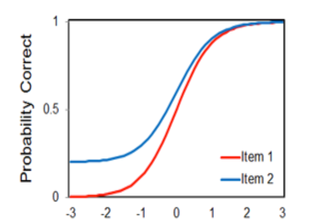
\includegraphics[scale=1.2]{Picture1.png}
\caption{Item Response Theory Demo}
\label{fig.1}
\centering
\end{figure}
You may refer the figure like Figure \ref{fig.1}.

\section{How to include tables?}
\begin{table}[H]
\begin{tabular}{|l|l|l|}
\hline
1 & 2 & 3 \\ \hline
4 & 5 & 6 \\ \hline
\end{tabular}
\caption{A Demo of Table}
\label{table.1}
\end{table}
You may refer the table like  Table \ref{table.1}. You can always find some online latex table generator or simply ask an AI for assistant in developing special needs of tabling formats.

\section{How to draw matrix?}

\begin{equation}
    A=\begin{bmatrix}
        1 & 2 \\
        3 & 4
    \end{bmatrix}
\end{equation}

\begin{equation}
    \det(A)=\begin{vmatrix}
        1 & 2 \\
        3 & 4
    \end{vmatrix}=-2
\end{equation}
\section{More on latex}

You need to double check your latex grammar before you start your thesis writing, please do google for what you want to know. This demo is not everything you need, only the basics.

\chapter{Simulation or Data Illustration}
These sections present the results of your research. The simulation section describes the experiments conducted using simulated or synthetic data, while the real data analysis section presents the results obtained from analyzing real-world data. Both sections should include a detailed discussion of the findings, highlighting any patterns, trends, or insights that emerge from the data. The length of these sections will depend on the amount of data analyzed and the complexity of the results.
\chapter{Discussion}
The discussion section is where you analyze and interpret the results of your research, connecting them to the broader context of your field. Here, you will explain the significance of your findings, compare them with existing literature, and discuss their implications.\\

{\bf Example:}

Summary of Key Findings:\\
In our study on the impact of social media usage on student mental health, we found that excessive use of social media was significantly correlated with increased levels of anxiety and depression among university students.\\

Interpretation and Significance:\\
These findings suggest that social media usage, when not managed appropriately, can have negative effects on mental health. This is particularly important given the widespread use of social media among young people today. Our results highlight the need for further research into the specific mechanisms linking social media use and mental health outcomes, as well as interventions to promote healthy social media habits.\\

Comparison with Literature:\\
Our findings are consistent with previous studies that have reported similar associations between social media use and mental health issues. However, our study adds to the existing literature by focusing specifically on university students and by using a larger and more diverse sample. This allows us to make more generalizable conclusions about the impact of social media on this particular population.\\

Implications:\\
The implications of our findings are twofold. First, they suggest that universities and educators should consider incorporating education on healthy social media usage into their curricula. Second, our results highlight the need for further research into the specific factors that contribute to the negative effects of social media on mental health, as well as the development of effective interventions to mitigate these effects.

\chapter{Conclusion}
The conclusion summarizes the main findings of your research, highlights the contributions of your study, and discusses the implications and limitations of your work. It should also suggest directions for future research. The conclusion should be concise and focused, typically around 200-300 words.\\

{\bf Example:}\\

In conclusion, this thesis has investigated the effectiveness of machine learning algorithms in predicting stock market trends. Our results indicate that LSTM networks outperform other algorithms in terms of accuracy and robustness. These findings suggest that LSTM networks have significant potential for use in practical stock market prediction systems. However, further research is needed to explore the impact of different hyperparameters and data preprocessing techniques on the performance of the models. Overall, this study contributes to the growing body of knowledge on machine learning for financial prediction and provides valuable insights for researchers and practitioners alike.\\


\newpage
\bibliography{ref_fyp.bib}{}
\bibliographystyle{siam}

\end{document}
